\documentclass{article}
\author{Jonathan Dyer}
\title{CS 1699: Privacy in the Electronic Society \\
        \textit{Project 1 -- Side-Channel Attacks}}

\usepackage{amsmath}
\usepackage{amsthm}
\usepackage{enumitem}
\usepackage[margin=0.8in]{geometry}
\usepackage{graphicx}
\usepackage[backend=bibtex,type=alphabetical,sorting=ynt]{biblatex}
\addbibresource{p1.bib}

% ============ USED FOR MY FORMAT ============
\newtheorem{thm}{Claim}
\providecommand{\task}[1]{\section*{Task #1}}
\providecommand{\soln}{\textbf{Solution: }}
\providecommand{\image}[1]{
    \begin{center}
        \includegraphics[width=1.0\textwidth]
            {#1}
    \end{center}
}
\providecommand{\tightlist}{
    \setlength{\itemsep}{0pt}\setlength{\parskip}{0pt}
}
\providecommand{\inlinecode}{\texttt}

% ============ USED FOR CODE LISTINGS ============
\usepackage{listings}
\usepackage[usenames,dvipsnames,svgnames]{xcolor}
\definecolor{javagreen}{rgb}{0.25,0.5,0.35}
\lstset{
    basicstyle          = \footnotesize,
    commentstyle        = \color{javagreen},
    frame               = single,
    language            = C,
    stringstyle         = \color{orange},
    numbers             = left,
    showstringspaces    = false,
    deletekeywords      = {len, max, format, min},
    morekeywords        = {yield, function, then, do, to},
    keywordstyle        = \color{blue},
    mathescape
}

\setcounter{secnumdepth}{0} % sections are level 1


\begin{document}
\maketitle

\tableofcontents

\section{Task W0}
\subsection{Problem P: String Comparison}
The problem chosen for this assignment is \textit{string comparison}, which involves checking one string for equality with another string.
This includes comparing both the \textbf{length} and the \textbf{content} of each string for a mismatch. \\
\textbf{Input:  } Two strings to be compared. \\
\textbf{Output: } Boolean indicating if the strings are \textit{equal}.

\section{Task W1}
\subsection{Relevance to Privacy}

String comparison has big implications in privacy for such a seemingly innocuous problem. Comparing values is a basic, necessary task for any system involving authentication or user input, which includes most (if not all) privacy-related services. This is especially true of web apps, and string comparison has been mentioned as a potential point of weakness on a number of online resources (more on how this weakness is exploited later). \cite{thisdata} \\
  \\
For example, an application may check if a username exists or a given password is correct by comparing its string value to the stored password for a user, whether in plaintext (unlikely for passwords) or by comparing their hash values. This typically occurs via a custom comparison for the object in question (potentially still timing sensitive!) or by using simple string comparison (both have been done historically). \cite{codahale} For example, the Java \inlinecode{MessageDigest.isEqual} method uses a simple byte comparison to check whether two digests are equal, which is essentially the implementation of string comparison for some languages.

\section{Task W4}
\subsection{Algorithm A: Break-on-Inequality}
Firstly, let's examine \textbf{Algorithm A} so that we can understand how and why this naive algorithm varies in runtime (including for inputs of the same size).
In the pseudocode below, first notice that if the strings are different lengths, a 'False' is returned immediately (lines 5-6).
This clearly changes the runtime in the case of different-sized inputs, which can reveal private information as discussed below.
More subtle is the character-by-character comparison, which breaks as soon as it finds a mismatch between the two strings (line 11). This reveals information about \textit{how} close the two strings are (or in the case of an attacker, how correct the guess was).

\begin{lstlisting}
// This method takes two strings, a and b, and returns True if they are equal, False otherwise
def algorithm_A (String a, String b)

  // First check that the lengths are the same
  if a.length != b.length
    return False

  // Now iterate through characters, comparing one by one
  int i = 0
  while i < a.length
    if a[i] != b[i]
      return False
    i = i+1

  // If we make it all the way, they match!
  return True
\end{lstlisting}


\subsection{Results}
Benchmarking \cite{benchmark} the above code -- implemented in the Ruby programming language -- over 1000s of iterations gives the results displayed in the table below. Note that the "different strings of the same length" differed in the first or nearly first characters while the "close strings of the same length" differed only on the final character, for both the sentence and the hash value. The following observations (about real time taken to compare inputs) are plain from the data:
\begin{itemize}\tightlist
  \item Comparing different strings of the same length is an order of magnitude slower than strings of different length.
  \item Comparing nearly-identical strings is \textit{another} order of magnitude slower.
  \item The difference between two close strings vs. two of the same string is very small, although it becomes more noticeable with a longer input.
\end{itemize}

\image{naive_results.png}

This may also be clearer from the following graph of the clock time taken by each comparison type. Notice that the difference between two different strings of the same length and two close strings is more dramatic as the length increases.

\image{naive_graph.png}


\subsection{Effect on Privacy}
It is clear that this measurable difference in string comparison times can be leveraged in a timing attack against some systems that make use of such an algorithm.
Although my first speculation was that such an attack could be used to recover a password from a system that allows multiple login attempts, I quickly recalled my computer science class on 'Privacy in the Electronic Society', wherein we learned that it is insecure and foolish to 1) transmit passwords in cleartext, or 2) store cleartext passwords on a secure system.
So the best that a timing attack could reveal in this instance (using techniques described below) is the hash of a password, or something that is normally sent in cleartext anyways.
But of course due to the cryptographic properties of any good hash function, recovering the password itself from such information is all but impossible. \cite{hash}
After further research and armchair rationalization, I determined that there are at least \textbf{two categories} of information that can be gained as a consequence of the above algorithm. The general setup for an attacker requires that:
\begin{enumerate}\tightlist
  \item The system being attacked makes use of Algorithm A, above.
  \item The attacker be able to choose the input to the algorithm (making this a \textit{chosen plaintext} attack).
  \item The attacker has some way of \textbf{verifying} whether or not the input was accepted; for example, a login form for a web app must indicate to the user (attacker) whether or not the input was correct, rather than simply sitting without any response.
\end{enumerate}

If the above conditions hold, then the system is functioning (loosely) as what is known as a \textit{verification oracle}, meaning that it will verify as correct or incorrect whatever input you provide, specifically by way of the (vulnerable) algorithm given above. This can leak information by way of a simple attack outlined here:

\begin{enumerate}\tightlist
  \item For any given set $x$ of known input characters and $y = {y_j \dots y_n}$ unknown, try every possibility for a variable $a$ in the input $x || a || y_{j+1} \dots y_n$ and some fixed filler, say \inlinecode{<underscore>}, for all $y_i \neq y_j$.
  \item Sample some dozens of times (or more if necessary, over a network, etc.) on each combination, and then take the mean (or median to mitigate outliers) of the time taken to return an error/False message.
  \item Set $a$ to be the character/byte with the greatest mean/median value (i.e. that takes the longest), add it to $x$, and then return to step 1 with $y = {y_{j+1} \dots y_n}$ and $a = y_{j+1}$.
\end{enumerate}
By repeating this process, first to find the correct length and then to find the correct combination of characters, it is possible to discern one or both of the following two types of (private) information.
This may require a more sophisticated timing software than Ruby's built-in benchmarking module (which I used), but I believe that it would not be difficult to achieve such an attack, even with a basic timing program.

\subsubsection{Existential information}
This type of information is leaked when an attacker exploits the timing differences in the above algorithm
to discover whether or not a system's stored list of information contains a given value. An attacker takes note of the typical response times for nonsense inputs and then compares them to response times for potentially legitimate input values. It is even simpler than the outline given above. An example will help to clarify:
\begin{itemize}\tightlist
  \item There is a web application called Foo Services that allows users to create accounts and login with an email address and password. It turns out that Foo uses Algorithm A to check the input email against valid emails to determine if such an account exists.
  \item The attacker, Mallory, creates an account with Foo Services. Mallory notices that when she mistypes her email in the login form, the Foo site displays an error: \inlinecode{Invalid username or password.}
  \item Mallory wants to discover if any of her friends have an account with Foo Services, so she follows the attack format given above, but instead of testing combinations of characters she simply cycles through her list of known email contacts, testing each several times (or dozens, or hundreds) and recording the average/median time that each takes to return the error message (obviously she doesn't know the password for any of their accounts, so she leaves that field blank for every attempt, or enters in an identical filler password for each attempt).
  \item Finally, Mallory enters her own email address (with the wrong password) and again tests several times to find the average/median time taken for a \textit{valid} account.
  \item According to the results section above, with enough samples Mallory should be able to tell which emails correspond to extant accounts. How? She can do this by noticing a (close to linear) boundary between those accounts that returned an error message more quickly and those accounts (including her own) which took longer. There may be some diffusion if some of the email addresses were similar to real accounts, but even that relationship should be distinguishable according to the results above.
  \item At this point Mallory has discovered which of her friends have accounts with Foo Services (with the email addresses she is aware of). She may leverage this information to perform a more targeted attack on one account (perhaps involving the password), or if Foo Services provides a sensitive or embarassing service, then the existence information itself is enough to compromise that individual's privacy.
\end{itemize}

Some variant of this attack is applicable in many circumstances. Some examples include checking "forgot my password" email tokens, testing answers to "security questions", or login forms as above. \cite{thisdata} Note that an attack similar to this could be perpetrated on older Unix systems, whose \inlinecode{login} program had a timing variation (execution of the \inlinecode{crypt} function) that depended on the string being recognized as a username. Combined with a dictionary attack on passwords, this could compromise the security of a system. \cite{wikitime} \\
  \\
This attack seems somewhat trivial, and perhaps only damaging in special circumstances. An extension of it that utilizes the full power of the attack outline first described would allow discovery of values that are associated with user information but typically hidden from users or inaccessible to outside attackers. It is this variant that we turn to next.

\subsubsection{Secret values}
This type of information is revealed when an attacker follows the iterative attack outline given previously. The examples I discuss all refer to hash values being uncovered, but there may be other applications I haven't considered or listed here. \\
  \\
  Suppose that there is a system, perhaps another web-based service, that authenticates users according to some keyed hash--a MAC or HMAC value for instance. This could be to authenticate a session cookie in a web browser \cite{codahale}, or to verify the author of some firmware for a system upgrade, or any other scenario wherein the hash of a password is used to confirm an identity. Also suppose that the three prerequisites defined at the beginning of this section all hold in relation to this hash value. That is:
  \begin{enumerate}\tightlist
    \item The system being attacked makes use of Algorithm A to compare the given authenticating hash value with the expected value.
    \item The attacker is able to choose the hash that is passed to the system to be verified.
    \item The system informs the user (attacker) of the results of that comparison in some way.
  \end{enumerate}
In other words, the system is functioning as a hash verification oracle for the attacker, who can pass arbitrary plaintext data along with a hash and in return find out whether or not they should "go together" (in the context of the system in question).
Thus, the attacker might the more advanced character-by-character attack that we outlined before to retrieve the corresponding hash for a given input data. It is provided again for convenience:
\begin{enumerate}\tightlist
  \item For any given set $x$ of known input characters and $y = {y_j \dots y_n}$ unknown, try every possibility for a variable $a$ in the input $x || a || y_{j+1} \dots y_n$ and some fixed filler, say \inlinecode{<underscore>}, for all $y_i \neq y_j$.
  \item Sample some dozens of times (or more if necessary, over a network, etc.) on each combination, and then take the mean (or median to mitigate outliers) of the time taken to return an error/False message.
  \item Set $a$ to be the character/byte with the greatest mean/median value (i.e. that takes the longest), add it to $x$, and then return to step 1 with $y = {y_{j+1} \dots y_n}$ and $a = y_{j+1}$.
\end{enumerate}
Now, retrieval of such a hash alone may not be explicitly detrimental to privacy, since (as mentioned before) it does not enable the recovery of a preimage/password -- at least for any hash function worth its "salt" (pun intended). \textbf{However}, certain attacks are facilitated specifically by having the hash of a value. Three particular examples are briefly described below, and further references are given.
\begin{enumerate}
  \item A straightforward attack known as "hash length extension" \cite{whitehathash} allows an attacker to falsely authenticate an "extension" of his choosing. This attack is valid for all Merkle-Damgard based hash algorithms, even for keyed hashes when the key is concatenated to the message (rather than an HMAC). A simple example is given at \cite{wikiexthash}.
  \item One attack, known as 'pass-the-hash', provides authentication to a system or service without the password for a given user, but just the hash. It applies on all systems using either the NTLM protocol or LanMan hash to authenticate users to the system. \cite{wikipasshash} Newer operating systems have disabled compromised versions of these protocols by default, but some of them continue to be used by third-party developers. If an attacker can acquire such a hash, then it would be possible to impersonate a user via a remote protocol such as SMB, FTP, HTTP, or others. The attack may be more sophisticated than our previous examples. Further reading: \cite{passhash}.
  \item Finally, and perhaps most \textbf{notably}, an actual timing attack involving hash-based authentication and string comparison was used to bypass a security measure in the Xbox 360 and modify system software (thereby enabling the running of custom software on the machine). This attack worked by exploiting time differences in verifying valid MAC values for kernel updates: for each valid byte in the hash, the system would reject about 2.2 milliseconds more slowly than an invalid byte in the equivalent position, enabling \textit{exactly our attack outlined above} to find a valid hash value. Details of this attack are presented in \cite{xbox}, and this and other MAC verification comparison timing attacks are mentioned in \cite{xboxbook}.
\end{enumerate}

There are other examples and resources besides the above elucidating the possibilities resulting from string comparison inconsistency. For example the popular crypto library developed by Google, known as Keyczar, fell prey to this problem in their HMAC verification implementation \cite{keyczar}, thus it is not unheard of even in well-developed libraries.

\pagebreak

\section{Task W7}
\subsection{Algorithm B: Constant-Time Comparison}
Now let's examine \textbf{Algorithm B} so that we can understand how and why this revised algorithm runs in a more constant-time manner, mitigating some of the effects discussed for Algorithm A above.
In the pseudocode below, first notice that before anything else we select a consistent number of iterations to run the byte-wise comparisons for (\inlinecode{len} in the code below, line 5)--this helps ensure that we don't reveal information about the length of the secret value (perhaps a login name), since that was an obvious and large timing difference in our naive algorithm.
Next, consider the revised loop through our inputs (lines 9-13). Rather than breaking this loop once we find a mismatch, we continue for the specified length \inlinecode{len} (line 9).
Then we check that both of the next characters are even valid to be compared (line 10). If so, we skip to the \inlinecode{else} (line 12) and proceed with the comparison. If either one is \textit{not} valid, we execute a "dummy" comparison to (hopefully) take the same amount of time as a real one (line 11).
Finally, we return the resulting boolean.

\begin{lstlisting}
// This method takes two strings, a and b, and returns True if they are equal, False otherwise
def algorithm_B (String a, String b)

  // We'll assume string a is the "system string" we're comparing the user-input against
  int len = a.length

  // Now set a boolean and then iterate through characters, comparing each (even on mismatch)
  boolean bool = (a.length == b.length)
  for i in $0 \dots$ len                  // for every character in the fixed length
    if a[i] == null || b[i] == null       // if we've reached the end of one string
      bool = (a[0] == a[0]) && bool       // compare something anyways
    else                                  // otherwise
      bool = (a[i] == b[i]) && bool       // compare the two chars, update the boolean

  return bool
\end{lstlisting}


\subsection{Results}
Benchmarking the above code -- implemented in Ruby -- over 1000s of iterations gives the results displayed in the table below. Note that the timing distinctions between the different types of comparison are almost entirely eliminated for shorter strings, and are statistically insignificant for longer strings/hash values. It is worth noting that comparing strings of different length still seems to be notably faster, especially for shorter inputs. This could reveal the length of a secret, given enough samples.

\image{constant_results.png}

The improvement is especially clear given the graph below, which shows much more even timing results across different types of input. In particular, the test on longer (hash) strings shows a slight reversal in the trend across strings of the same length--which could indicate that it would lead an attacker to make incorrect guesses (a desirabe trait).

\image{constant_graph.png}

\subsection{Trade-Offs \& Design Decisions}
There is a significant performance cost associated with making constant-time comparisons, especially when trying to obscure even the length of the secret value(s). Notice in the comparison graph below for Naive vs. Constant Comparison that the constant-time algorithm takes nearly twice as long when comparing similar strings and \textit{several times} as long when comparing very different strings. This would be a highly significant cost on a system or web-server that may receive thousands of requests a day/hour/minute. \par

\begin{center}
    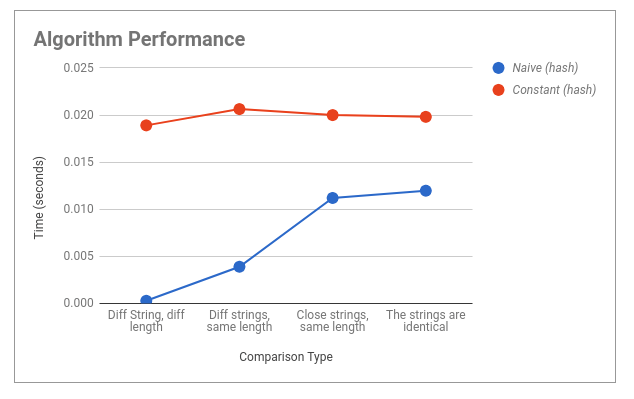
\includegraphics[width=0.8\textwidth]
        {alg_perf.png}
\end{center}


Additionally, not all the timing difference for comparing strings of different length is mitigated. This could be because the 'else' conditional code (lines 12-13) is not being executed for every null character of the compared string, resulting in faster overall execution. Some amount of randomness could perhaps be introduced that would further obscure those lines of comparison. \par

Finally, because the chosen amount of time is based on the \textit{first} string passed to the algorithm, we risk revealing length of secret values anyways if our implementation is known and the attacker can duplicate our system/working environment.
An alternative to this would be to always go with the longer string, but that might open up the algorithm to DOS (denial-of-service) attacks, where the attacker simply passes excessive input. This could be checked for, but length information could be revealed by passing very short arguments and working up to the secret string length. On the other hand, if we choose to always go with the shorter string, the inverse process would also reveal lengths.
One solution to this problem may be to choose a random \inlinecode{len} value within an acceptable range and iterate for that many bytes (but this may not mitigate all leakage). \\

\section{Task W8}
\subsection{Remaining Problems}
There is still potential to leak lengths of secret values (as mentioned in the trade-offs section). There are likely better ways to obscure those lengths that I have not implemented above, without sacrificing quite as much in performance. One option is randomizing the number of byte-comparison iterations as suggested above. However, it is plain that there will always be a performance cost associated with implementing a constant-time algorithm (since we can only come \textit{up} to the slowest time, rather than decreasing everything else).\\
 \\
It is also possible that the very timing attack described above could work with my new and improved algorithm, perhaps with more samples. This would require a more detailed and granular timing software, probably written in a lower-level language (e.g. C), but would almost certainly still be possible for a dedicated attacker -- especially given the comparison graph above, which still reveals some variation.\\
 \\
It is clear that ensuring no information is leaked by a string comparison algorithm is a nontrivial task. We've learned not only that, but that this task is in fact important to securing applications and systems that involve private information. Better implementations should be (and are more frequently) included in complete and well-tested cryptographic libraries.

\pagebreak

\printbibliography[heading=bibintoc]

\end{document}
